\documentclass[compress]{beamer}
\usepackage{ifthen}

\title{Track-based Alignment of the Muon Chambers: Status and Schedule}
\author{Jim Pivarski}
\institute{Texas A\&M University}
\date{ 5 December, 2006}

\setbeamertemplate{navigation symbols}{}
\setbeamertemplate{headline}{\includegraphics[height=1 cm]{../cmslogo} \hspace{0.1 cm} \includegraphics[height=1 cm]{../tamulogo} \hfill
\begin{minipage}{9 cm}
\vspace{-0.75 cm} \small
\begin{center}
\ifthenelse{\equal{\insertpagenumber}{1}}{}{\insertsection}
\end{center}
\end{minipage} \hfill
\begin{minipage}{1 cm}
\vspace{-0.75 cm} \small
\begin{center}
\ifthenelse{\equal{\insertpagenumber}{1}}{}{\insertpagenumber/\pageref{numpages}}
\end{center}
\end{minipage}}

\xdefinecolor{verylightgray}{rgb}{0.95,0.95,0.95}
\beamertemplateshadingbackground{verylightgray}{white}

\begin{document}
\frame{\titlepage}
\section*{Track-based Muon Alignment --- Jim Pivarski}

\begin{frame}
\frametitle{Comparison with Hardware Alignment}

\begin{description}
\item[Track-based alignment:] vary chamber positions to minimize $\sum |$residual$|^2$ (that is, $\sum |$track $-$ hit position$|^2$)
\end{description}
\begin{itemize}
\item<1-> requires a large dataset ($\gg$ 2007 run, $\sim$a day full luminosity)
\item<2-> insensitive to translations along line of sight from IP
\item<3-> cannot recover trigger inefficiency due to misalignment
\item<4-> the final alignment
\end{itemize}

\vfill
\begin{description}
\item[Hardware alignment:] physical sensors on the chambers
\end{description}
\begin{itemize}
\item<1-> sensitive to short timescales
\item<2-> geometry is not radial: compliments track-based
\item<3-> can correct misalignments before data-taking
\end{itemize}
\end{frame}

\begin{frame}
\frametitle{HIP: a Simple Alignment Algorithm}

\begin{itemize}
\item Advantage: easy to see what's happening (diagnostic plots)
\end{itemize}

\vspace{0.3 cm}
{\small $r_x$ $=$ track$-$hit residual in local coordinate $x$}

\vspace{-0.75 cm}
\begin{center}
\begin{tabular}{p{0.31\linewidth} p{0.31\linewidth} p{0.31\linewidth}}
  \begin{minipage}{\linewidth}
    \includegraphics[width=\linewidth]{dof_x}
  \end{minipage} &
  \begin{minipage}{\linewidth}
    \includegraphics[width=\linewidth]{dof_y}
  \end{minipage} &
  \begin{minipage}{\linewidth}
    \includegraphics[width=\linewidth]{dof_z}
  \end{minipage} \\
  \begin{minipage}{\linewidth}
    \begin{center}
      $x$: offset in $r_x$
    \end{center}
  \end{minipage} &
  \begin{minipage}{\linewidth}
    \begin{center}
      $y$: offset in $r_y$
    \end{center}
  \end{minipage} &
  \begin{minipage}{\linewidth}
    \begin{center}
      $z$: inaccessible
    \end{center}
  \end{minipage} \\
  & & \\
  \begin{minipage}{\linewidth}
    \tiny
    \includegraphics[width=\linewidth]{dof_phix} \\ \mbox{ }
  \end{minipage} &
  \begin{minipage}{\linewidth}
    \tiny
    \includegraphics[width=\linewidth]{dof_phiy} \\ \mbox{ }
  \end{minipage} &
  \begin{minipage}{\linewidth}
    \tiny
    \includegraphics[width=\linewidth]{dof_phiz} \\ \mbox{ }
  \end{minipage} \\
  \begin{minipage}{\linewidth}
    \begin{center}
      $\phi_x$: $r_y$ linear in $y$ \\ \mbox{ }
    \end{center}
  \end{minipage} &
  \begin{minipage}{\linewidth}
    \begin{center}
      $\phi_y$: $r_x$ linear in $x$ \\ \mbox{ }
    \end{center}
  \end{minipage} &
  \begin{minipage}{\linewidth}
    \begin{center}
      $\phi_z$: $r_x$ linear in $y$ and $r_y$ linear in $x$
    \end{center}
  \end{minipage} \\
  \begin{minipage}{\linewidth}
    \scriptsize
    \begin{center}
      (slope $=$ $1 - \cos\phi_x$)
    \end{center}
  \end{minipage} &
  \begin{minipage}{\linewidth}
    \scriptsize
    \begin{center}
      (slope $=$ $1 - \cos\phi_y$)
    \end{center}
  \end{minipage} &
  \begin{minipage}{\linewidth}
    \scriptsize
    \begin{center}
      (slope $=$ $\sin\phi_z$)
    \end{center}
  \end{minipage}
\end{tabular}
\end{center}
\end{frame}

\begin{frame}
\frametitle{History of Our Involvement}

\begin{description}
\item[3 October:] Announced our involvement at Purdue EMU meeting
\item[20 October:] Could arbitrarily move detector elements in CMSSW
\item[22 October:] Could calculate residuals
\item[26 October:] Proposed MuonAlignmentAnalyzer to AlCaReco
\item[] They convinced us to extend CommonAlignment
\item[13 November:] Presented at PRS/mu
\end{description}

\hspace{-0.8 cm}
\begin{minipage}{\linewidth}
\begin{tabular}{p{0.6\linewidth} p{0.5\linewidth}}
%% \begin{minipage}{\linewidth}
%% \begin{center}
%% \hspace{-1 cm} We can move detectors
%% \end{center}
%% \end{minipage} &
%% \begin{minipage}{\linewidth}
%% \begin{center}
%% \hspace{-0.5 cm} We can calculate residuals
%% \end{center}
%% \end{minipage} \\
\begin{minipage}{\linewidth}
  \includegraphics[width=\linewidth]{misalignment_analyzer}
\end{minipage} &
\begin{minipage}{\linewidth}
  \hspace{-0.5 cm}
  \includegraphics[width=\linewidth]{all_residuals}
\end{minipage}
\end{tabular}
\end{minipage}

\end{frame}

\begin{frame}
\frametitle{CommonAlignment}

\begin{itemize}
\item Three alignment algorithms are sub-modules of CommonAlignment,
including HIP (called CSA06Alignment)
\item Designed for tracker and muon chambers, but only implemented for
tracker
\end{itemize}

\begin{center}
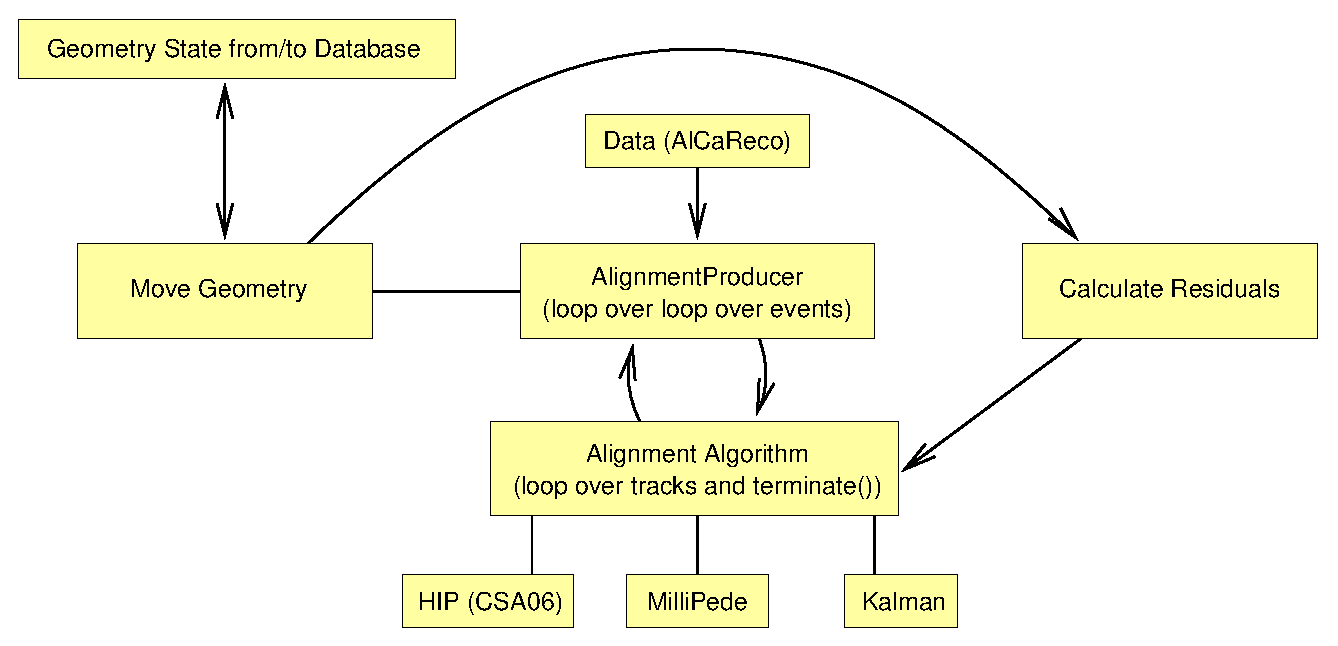
\includegraphics[width=\linewidth]{flow_chart_simplified}
\end{center}
\end{frame}

\begin{frame}
\frametitle{Current Status}

\begin{itemize}
\item Can edit and update muon geometry (works in local area)
\item Can calculate trajectory of tracker-fitted tracks at muon hits
and put this into the Event in a standard way
\item Need to modify CommonAlignment to get this object and \mbox{use it} to
calculate residuals
\end{itemize}

\begin{center}
\includegraphics[width=\linewidth]{flow_chart}
\end{center}
\end{frame}

\begin{frame}
\frametitle{Schedule through next year}

\renewcommand{\arraystretch}{1.5}
\begin{tabular}{p{0.18\linewidth} p{0.75\linewidth}}
Deadline & Task \\ \hline

1 Jan, \hfill 2007 & Finish integrating muon chambers into alignment framework \\

1 Mar, \hfill 2008 & Transition CSA06Alignment to HIPAlignment and
develop low-level diagnostics suite \\

1 Apr & Prototype and study realistic alignment procedure, assuming a
source of muons \\
 
1 May & Evaluate possible sources ($W\to\mu\nu$, $Z\to\mu\mu$,
cosmics, or good muon) and finalize routine \\

1 Jun & Document everything
\end{tabular}
\end{frame}

\begin{frame}
\frametitle{How much data do we need?}

\begin{itemize}
\item Start with CMS NOTE 2006/016 toy MC (``for illustrative purposes only!'')
\item Distinguish between barrel and endcap: intrinsic resolutions,
overlapping geometry, $\eta$ distribution of $W\to\mu\nu$ and $Z\to\mu\mu$
\item Simulate multiple scattering, non-uniform $\vec{B}$, propagated
from tracker (30\% effect)
\end{itemize}

\vfill
2 days of $10^{30}/$cm$^2/$s at 0.9 TeV:

\vspace{-0.25 cm}
\begin{center}
4--6 mm resolution in barrel, 3--4 mm in endcap
\end{center}

\vfill
$10^{33}/$cm$^2/$s at 14 TeV:

\vspace{-0.25 cm}
\begin{center}
17 hours for 200-300 $\mu$m in barrel (410,000 muons), \\ 10 hours for 100-150 $\mu$m in endcap (220,000 muons)
\end{center}
\end{frame}

\begin{frame}
\frametitle{Summary}

\begin{itemize}\setlength{\itemsep}{0.35 cm}
\item We are implementing a simple, robust alignment algorithm that
provides opportunities for diagnostics

\item Software development is progressing smoothly (well-designed
infrastructure)

\item Conservative schedule has an alignment routine ready on time

\item Track-based alignment cannot be precise with 2 days of
low-energy, low-luminosity data

\item At full energy and luminosity, track-based can be sensitive to
timescales as short as a day
\end{itemize}

\label{numpages}
\end{frame}

\begin{frame}
\frametitle{How much data do we need?}

MB1 alignment resolution {\it per track} (scales with $1/\sqrt{N_{\mbox{\scriptsize track}}}$)

\vfill
\begin{tabular}{p{0.55\linewidth} p{0.4\linewidth}}
  \begin{minipage}{\linewidth}
    \vspace{0.25 cm}
    global translations:

    \begin{center}
      \begin{tabular}{c c c}
	\textcolor{red}{$rphi$} & $R$ & \textcolor{red}{$z$} \\\hline
	\textcolor{red}{8 mm} & 80 mm & \textcolor{red}{8 mm}
      \end{tabular}
    \end{center}
  \end{minipage} &
  \begin{minipage}{\linewidth}
    \begin{center}
      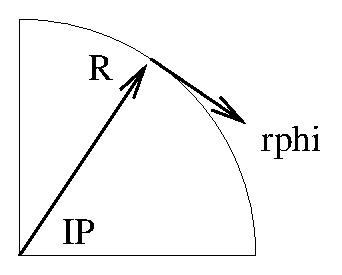
\includegraphics[height=1.7 cm]{global_coordinates}
    \end{center}
  \end{minipage} \\
  & \\
  \begin{minipage}{\linewidth}
    \vspace{0.25 cm}
    local rotations:

    \begin{center}
      \begin{tabular}{c c c}
	$\phi_x$ & $\phi_y$ & \textcolor{red}{$\phi_z$} \\\hline
	70 mrad & 50 mrad & \textcolor{red}{10 mrad}
      \end{tabular}
    \end{center}
  \end{minipage} &
  \begin{minipage}{\linewidth}
    \begin{center}
      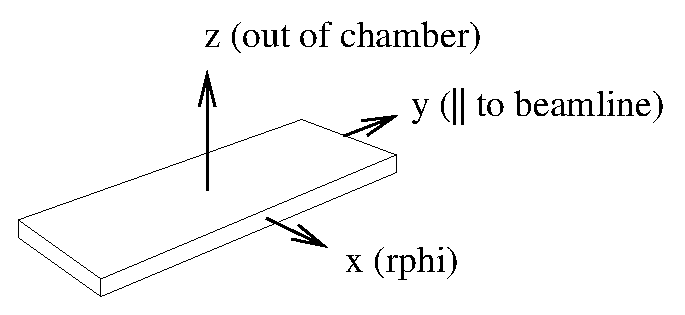
\includegraphics[height=2 cm]{coordinates}
    \end{center}
  \end{minipage} \\
\end{tabular}

\vspace{0.75 cm}
\textcolor{red}{*direct effect on tracking}

\end{frame}

\begin{frame}
\frametitle{How much data do we need?}

$\left.
\mbox{\begin{minipage}{0.8\linewidth}
\vspace{-\baselineskip}
\begin{eqnarray*}
  rphi &\to& \mbox{8 mm $x$-residual} \\
  \phi_z \times L_y &\to& \mbox{25 mm $x$-residual at chamber edge} \\
  \mbox{global } z &\to& \mbox{8 mm $y$-residual} \\
  \phi_z \times L_x &\to& \mbox{20 mm $y$-residual at chamber edge}
\end{eqnarray*}
\end{minipage}}
\right\} \textcolor{red}{\mbox{15-20 mm}}$

\vspace{0.35 cm}
\textcolor{red}{for all barrel chambers} (independent of chamber lengths)

\vfill
Intrinsic resolutions of $\displaystyle \frac{\mbox{endcap}}{\mbox{barrel}} = \frac{\mbox{50 $\mu$m}}{\mbox{170 $\mu$m}}$
\hfill \begin{minipage}{3 cm}
\small (E.\ Torassa, {\it Review of the CMS Muon Detector System})
\end{minipage}

\vfill
\textcolor{red}{5-6 mm for all endcap chambers}

\end{frame}

\begin{frame}
\frametitle{How much data do we need?}

Toy MC was for innermost muon chamber: what about resolution loss in
outer chambers?  Full simulation:

\begin{center}
\includegraphics[width=0.7\linewidth]{degradation_of_residuals3}
\end{center}

\vspace{-0.3 cm}
Multiple scattering, non-uniform $\vec{B}$, propagated from tracker
$\Rightarrow$ 30\% widening of distribution
\end{frame}

\begin{frame}
\frametitle{How much data do we need?}

To get 200-300 $\mu$m in barrel and 100-150 $\mu$m in endcap,

\vspace{-0.5 cm}
\[ \left(1.3 \, \frac{\mbox{20 mm}}{\mbox{300 $\mu$m}}\right)^2 = \mbox{6800}\,\frac{\mbox{muons}}{\mbox{DT}} \mbox{\hspace{0.6 cm}} \left(1.3 \, \frac{\mbox{6 mm}}{\mbox{150 $\mu$m}}\right)^2 = \mbox{2700}\,\frac{\mbox{muons}}{\mbox{CSC}} \]

$\times$ 60 {\small non-overlapping} $=$ 410,000 barrel \mbox{\hspace{0.5 cm}} $\times$ 80 $=$ 220,000 endcap

\vfill
At 0.9 TeV:

\vspace{-0.75 cm}
\begin{eqnarray*}
\mbox{\hspace{0.3 cm}} 2 \times \sigma(Z) \times {\mathcal B}(\mu\mu) \times \epsilon(\eta) &=& \mbox{0.14 nb (barrel), 0.060 nb (endcap)} \\
\sigma(W) \times {\mathcal B}(\mu\nu) \times \epsilon(\eta) &=& \mbox{0.67 nb (barrel), 0.29 nb (endcap)}
\end{eqnarray*}

\vfill
At 14 TeV:

\vspace{-0.75 cm}
\begin{eqnarray*}
2 \times \sigma(Z) \times {\mathcal B}(\mu\mu) \times \epsilon(\eta) &=& \mbox{1.2 nb (barrel), 1.2 nb (endcap)} \\
\sigma(W) \times {\mathcal B}(\mu\nu) \times \epsilon(\eta) &=& \mbox{5.4 nb (barrel), 5.4 nb (endcap)}
\end{eqnarray*}
\end{frame}

\end{document}
